%   File: Golfer.tex
% Author: Adam Leeper
%------------------------------------------------------------------------------
%\\[0.45pc]
\providecommand{\isolatedBuild}[1]{#1}% Fallback definition to build normally.
\isolatedBuild{
  \documentclass[11pt,letterpaper]{book}
  %\documentclass[11pt,letterpaper]{book}

% aleeper: I think these are needed for Paul's macros?
\usepackage{epsfig}
\usepackage{epstopdf}

%\makeatletter
%\typeout{The import path is \import@path}
%\makeatother

\usepackage{import}

\subimport{./}{packagesMitiguy.sty}
\subimport{./}{macrosMitiguy.tex}
\subimport{./}{PageStylesMitiguy.tex}
\subimport{./}{macrosLeeper.tex}
   % Found via TEXINPUTS environment variable.
  \isolatedBuildHeader{Velocity Constraints and Rolling}
                      {Amusement Park: Ship Ride}
}
%%%
%%%
%%%
{
\small
\begin{minipage}[t]{1.0\linewidth}
%  \minipageTopAnchor
  A common theme-park ride is pictured below.
  The ride features a ship, \basis{B}, that swings from a top support, $B_o$,
  fixed in a Newtonian reference frame \basis{N}, as pictured.
  A tire \basis{A}, whose center \origin{A} is fixed in \basis{N}, makes contact
  with the bottom of the ship.
  Hence, the angular motion of the tire is used to swing the ship back and
  forth.
  %
  \\[0.45pc]
  During a certain interval, the \textbf{counter-clockwise} rotation rate of
  the tire is described by $\omega_A = 10 \mult \sin(t)$.
  Let the \textbf{counter-clockwise} rotation rate of the ship be denoted by
  $\omega_B$.
  \\[0.45pc]
  The radius of the tire is $R_A = 0.3$ m, and the distance from \origin{B} to the
  bottom surface of the ship is $R_B = 6$ m.
  %
  %\\[0.45pc]
  %Right-handed orthogonal unit vectors \uvecxyz{n} are fixed in \basis{N}
  %as shown.
  %
  \begin{center}
    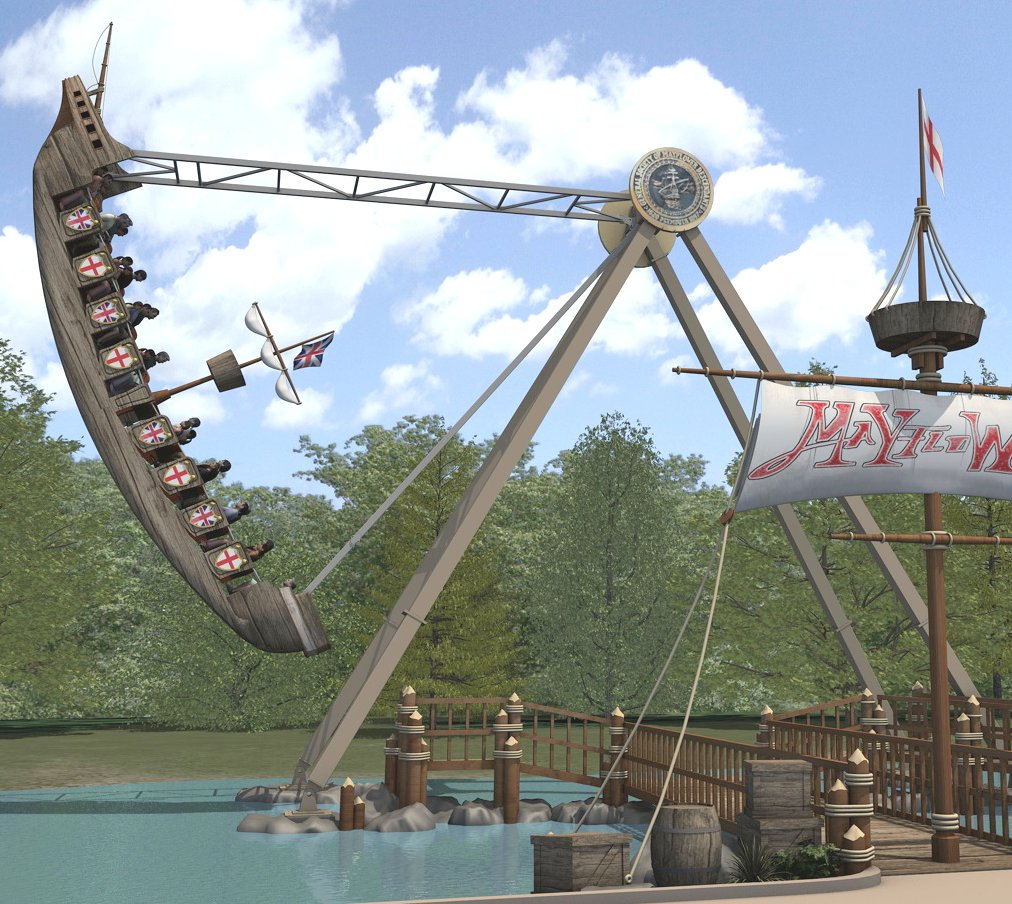
\includegraphics[height=6cm]{mayflower.jpg}
    \hspace{1cm}
    \includegraphicsAB[height=6cm]{boat-solution.png}{boat.png}
  \end{center}
  %
  \begin{enumerate}
    \item \textbf{Calculate} the velocity of the point of the tire in contact
      with the ship, $\vel{\contactPoint{A}{B}}{N}$, and calculate the velocity of the point of
      the ship in contact with the tire, $\vel{\contactPoint{B}{A}}{N}$.
      %
      \\[0.45pc]
      \Solution{}{0.99\linewidth}{
        \begin{tabular}{@{}l@{ \equals[\;] }l}
          $\vel{\contactPoint{A}{B}}{N}$
          & $\vel{\origin{A}}{N}\plus \angvel{A}{N}
          \CrossProduct \posvec{\origin{A}}{\contactPoint{A}{B}}$
          \\[0.45pc]
          & $\zerovec \plus (\omega_A \uvecz{n})
          \CrossProduct (R_A \uvecy{n})$
          \\[0.45pc]
          & $\omega_A R_A(\minus \uvecx{n})$
        \end{tabular}
        \hspace{1cm}
        \begin{tabular}{@{}l@{ \equals[\;] }l}
          $\vel{\contactPoint{B}{A}}{N}$
          & $\vel{\origin{B}}{N}\plus \angvel{B}{N}
          \CrossProduct \posvec{\origin{B}}{\contactPoint{B}{A}}$
          \\[0.45pc]
          & $\zerovec \plus (\omega_B \uvecz{n})
          \CrossProduct (\minus R_B \uvecy{n})$
          \\[0.45pc]
          & $\omega_B R_B(\uvecx{n})$
        \end{tabular}
        \\[1.0pc]
      }
	    %
    \item When the ship \textbf{rolls} on the tire, write the relevant
      \textbf{constraint equation} and use it to find a \textbf{scalar}
      relationship between $\omega_A$ and $\omega_B$.
      %
      \\[0.45pc]
      \Solution{}{0.99\linewidth}{
        \begin{tabular}{l@{}r@{\equals[\;]}l}
          Rolling Constraint:
          & $\vel{\contactPoint{A}{B}}{N}$
          & $\vel{\contactPoint{B}{A}}{N}$
          \\[0.45pc]
          & $\minus \omega_A R_A \uvecx{n}$
          & $\omega_B R_B \uvecx{n}$
          \\[0.45pc]
          dot with $\uvecx{n}$:
          & $\minus \omega_A R_A$
          & $\omega_B R_B$
        \end{tabular}
      }
      %
    \item \textbf{Compute} $\omega_B$ and $\alpha_B$ when $t = \frac{\pi}{6}$
      seconds.
      %
      \\[0.45pc]
      \Solution{}{0.99\linewidth}{
        The rolling constraint gives us one useful equation. We can get another
        one by implicit differentiation:
        $$\minus \omegadot_A R_A \omegadot_B R_B
          \text{\symmetricSpace{1cm}{or}}
          \minus \alpha_A R_A \alpha_B R_B$$
        %
        We are given $\omega_A = 10 \sin(t)$. Taking the derivative with respect
        to time yields:
        %
        $$\omegadot_A = 10 \cos(t)
          \text{\symmetricSpace{1cm}{or}}
          \alpha_A = 10 \cos(t)$$
        %
        So plugging in:
        \\[0.45pc]
        \begin{tabular}{r@{\equals[\;]}l}
          $\omega_B (t = \frac{\pi}{6})$
          & $\minus \frac{R_A}{R_B} \omega_A (t = \frac{\pi}{6})$
          \\[0.45pc]
          & $\minus \frac{0.3 m}{6 m} (10 \sin(\frac{\pi}{6}))$
          \\[0.45pc]
          & $\minus 0.25 \frac{rad}{s}$
        \end{tabular}
        \hspace{1cm}
        \begin{tabular}{r@{\equals[\;]}l}
          $\alpha_B (t = \frac{\pi}{6})$
          & $\minus \frac{R_A}{R_B} \alpha_A(t = \frac{\pi}{6})$
          \\[0.45pc]
          & $\minus \frac{0.3 m}{6 m} (10 \cos(\frac{\pi}{6}))$
          \\[0.45pc]
          & $\minus 0.43 \frac{rad}{s^2}$
        \end{tabular}
      }
      %
  \end{enumerate}
\end{minipage}
}
%
\isolatedBuildFooter